\chapter{Literature Review}

The following chapter blah blah blah...

\section{Data Stream}

Golab and Ozsu define data stream as "a real-time, continuous, ordered (implicitly by arrival time or explicitly by timestamp) sequence of items. It is impossible to control the order in which items arrive, nor is it feasible to locally store a stream in its entirety". \cite{golab2003issues}

\subsection{Comparison to a Database Management System (DBMS)}

Historically, data has been stored into database management systems (DBMS) where it was later analysed the assumption being that there would be enough disk space to contain the data. This approach fits many purposes but recently applications started "feeling the need" to analyse rapidly changing data on-the-fly.

This has brought on an advent of data stream processing. Several stream-processing frameworks have emerged such as Apache Storm \cite{ApacheStorm}, Apache Spark \cite{ApacheSpark}, and Onyx \cite{Onyx}. These frameworks, usually ran on a cluster, provide the user with abstractions which greatly simplify writing a real-time data stream processing application.

Whereas DBMSs excel at getting an exact answer to a query, data streams usually provide an approximate answer. The answer is approximate because it is usually correct only within a certain window of time, the query is simplified because it can only be ran in one pass, or because it is used with a sampling rate which does not include all events. A typical data stream analysis using windows and sampling is depicted in figure \ref{fig:stream}.

The assumption behind using a time window is that users are most likely interested in the most recent events. That way they can  react to change quickly. Sampling on the other hand is used to reduce the number of events used for a query. \cite{Gaber:2005:MDS:1083784.1083789}

\begin{figure}[!htb]
	\centering
	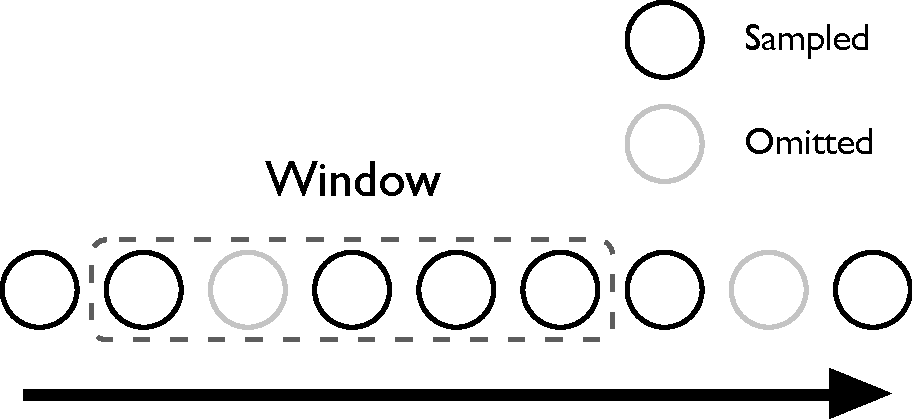
\includegraphics[scale=0.5]{pdf/stream.pdf}
	\caption{Stream Querying.}
	\label{fig:stream}
\end{figure}

Even though the answer might only be approximate it can have great value because the query is answered at the right time. Furthermore, even though the query may run only on a subset of data it is still possible to detect trends or system failures. For example, Twitter are using Apache Storm to run real-time analysis on millions of events per second for their analytics product. \cite{Solovey}

In research, several techniques have been developed to enable real time data stream mining. For example, the MOA environment \cite{Bifet:2010:MMO:1756006.1859903} which enables real time machine learning using the WEKA machine learning workbench \cite{Holmes1994}.

\section{Apache Storm}

\todo{What is Storm}

Apache Storm is an open source distributed real-time computation system. Storm was Originally created by Nathan Marz while working at BackType. \cite{NathanAbout} BackType was later acquired by Twitter which is when Storm became open source.

\todo{Who uses Storm}

Storm is reportedly used by 81 companies listed on their website \cite{https://storm.apache.org/documentation/Powered-By.html} and possibly many others. 

\todo{What research has there been on Storm}

\section{Ports to Multi-core}

\section{Similar Efforts}

\todo{Has anyone ported Storm somewhere}

\todo{Real time on multi-core}

\todo{What has been ported}

\section{Summary}